\section{Low Level Vision - Biological}

\subsection{Human Visual System}
After the retina, the signals pass through the optic nerve to the \emph{Lateral Geniculate Nucleus}, then to the \emph{Primary Visual Cortex} in the cerebral cortex of the brain.

\subsubsection{Left is Right}
The right visual field is projected to the left side of each retina and vice versa. Both left sides connect to the left LGN, and both right to the right LGN - so the \textbf{rightvisual field} is in the \textbf{left LGN}, rather than the left eye (same for the right side). \\
This can be seen in the below image (taken from the slides): \\

\begin{figure}[H]
    \centering
    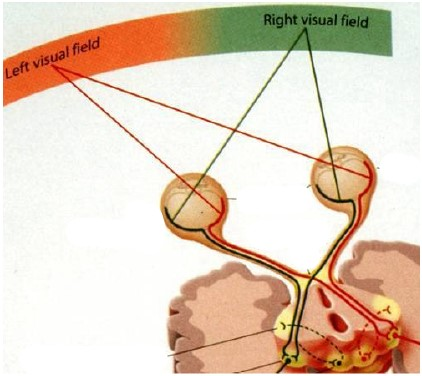
\includegraphics[width = \textwidth, height=7cm,keepaspectratio ]{Images/Visual_Field_to_LGN}
\end{figure}

\subsubsection{Lateral Geniculate Nucleus}
The section between the optic nerve and the brain. It's mostly considered a relay station consisting of centre-surround cells, but some recent research says that some computation occurs. It's unknown what this computation is. 

\subsubsection{Cerebral Cortex}
All higher processing functions of the brain happen here - 2\% of the body mass, 20\% of the body's energy consumption. It's divided into specialised areas - there are approx. 30 for vision, approx. 50\% of the total volume. \\

The vision system in the cerebral cortex can be roughly split into two paths:
\begin{enumerate}
    \item Where - actual vision processing (spatial, colour, motion)
    \item What - classification and understanding
\end{enumerate}
Both paths begin in the V1/striate cortex (primary visual cortex, simple/local receptive fields), then move to more specialised areas with larger receptive fields.

\subsection{V1 cells}
V1 cells have small receptive fields, but have more receptive properties than gangilon/LGN cells, including: orientation, position, direction of motion, colour, binocular disparity and eye of origin. 

\subsubsection{Colour - Double Opponent cells}
Same structure (slightly larger) than centre-surround cells, but specifically look for colour changes/boundaries.e.g. red centre/green surround

\subsubsection{Orientation - Simple/Complex/Hyper-complex Cells}
Simple V1 cells respond most strongly for a gradient in a particular direction/orientation/ contrast/position in the field - these act as edge/bar detectors. \\

Complex Cells are like simple, but are more tolerant with contrast/position - still highly orientation selective. These also act as edge detectors, with some flexibility on location.\\

Hyper-complex cells are like complex, but also depend on the length of the stimulus (length of the edge, not the width). If the stimulus is too long/short, responds weakly. Both complex/hyper-complex are good for motion detection.

\subsubsection{Spatial Frequency}
Most V1 cells are tuned to a particular spatial frequency (contrast), and respond most strongly to it. Their response drops to almost zero above this frequency, and slowly grows to maximum below it. 

\subsubsection{Eye of Origin}
\emph{Monocular Cells} only recieve input from one eye: retinal, LGN and some V1 cells.\\

\emph{Binocular Cells} receive input from both eyes. They have a separate identical field for each eye, and if both fields have the same response then the cell sends a strong response. This can be used to calculate depth of a stimulus: the disparity (distance) between the stimulus in each eye is inversely proportional to the depth. 

\subsubsection{Hypercolumnns}
V1 cells are grouped into hypercoloumns, based on where in the retina their receptive fields are. Each contains all the cells needed for one section: colour, orientation,etc. in approx 1mm$^2$. \\

The columns are arranged \emph{retinotopically} - adjacent hypercolumns correspond to adjacent sections on the retina. There are more hypercolumns for the fovea, as there are more gangilons/photoreceptors on the fovea. 

\subsection{Gabor Functions}
The receptive fields(RFs) of simple cells act similarly to Gabor Functions (Gaussian x Sinusoid function). These functions have five parameters:
\begin{enumerate}
    \item $\sigma$ - Scale of the gaussian - the variance/size of the RF in the mask
    \item $f$ - Frequency of the sinusoid - number of alternating regions in the RF
    \item $\Psi$ - Phase of the sinusoid - whether the RF starts with an 'on' or 'off' section
    \item $\theta$ - Orientation of the RF 
    \item $\gamma$ - Spatial aspect ratio of the RF
\end{enumerate}

\subsubsection{Convolutions}
Convolving an image with a single gabor mask gives the results of the simple cell at each position (Each hypercolumn). Convolving with multiple gabor cells (with different phases) and taking the strongest response mimics a complex cell (invariant to contrast) - this can also be obtained with a $\sqrt{sum}$ of two masks with opposing phase (Energy Model).\\

By varying both the phase and the orientation, we can detect edges in multiple orientations. 

\subsubsection{Continuous Wavelet Transform}
To detect edges at multiple scales, we also have to vary $\sigma$. Convolving a signal(image) with similar masks at different frequencies/scales is called a \emph{continuous wavelet transform} - in this case, the wavelet is the gabor.

\subsection{Image Components}
Images/templates can be thought of as a super-position of various components/elementary features, such as lines or circles. Each component can be weighted (0 if not present), to make any image a weighted sum of a set of components. i.e
\begin{center}
    $A \cdot y = x$ \\
    where A is a m by n matrix of image components, y is a n by 1 vector of weights, and x is a m by 1 vector representing a flattened image
\end{center} 
This technique can be used to represent multiple images with the same set of components, by making y and x into n by p matrices (p is the number of images). Finding A and y for a set of p images is an ill-posed problem, that can be solved (under certain constraints) by some matrix factorisation methods. \\

\subsubsection{Natural Image Components}
Gabor functions work well as natural image components - the brain is able to combine them to represent most images. They're also fairly efficient - most images only weight a few components (\emph{sparsity constraint} to represent images with as few weights as possible), so only a few neurons fire which gives efficient coding. \\

\subsubsection{Applications of Image Components}
A similar tactic is used in Jpeg image compression, which uses cosines rather than gabors. It doesn't have a sparsity constraint, but this is still more efficient that storing the whole image. The image is split into patches, each of which is given separate activation weights. \\

By replicating the image using gabor functions, high frequency data is often lost - this can be used to reduce the noise of the image (\emph{image denoising}). Missing sections of the picture can also be reconstructed by replicating the image (\emph{image inpainting}). 

\subsection{Non-Classical RFs}
The classic receptive field of a neuron is the area of the image/visual field that it responds to. However, in the V1/striate cortex, this response can be affected by the responses from other neurons (context) - the RFs of these neurons are called the non-classical RF. \\

Co-linear/ Co-circular neighbours (not just adjacent) excite a neuron, parallel neighbours inhibit it. These connections are called the \emph{Assosciation field} - they only enhance/reduce the response, and cannot trigger a response from the neuron if its own RF is empty. \\

Enhancing/exciting a response makes it easier to see elements that are aligned (smooth contours vs. background noise). Inhibiting similar elements allow outliers to 'pop out' and be easier to see (odd items/boundaries between regions). Both of these contribute to edge detection.  